\documentclass[12pt,a4paper]{article}

\usepackage[utf8]{inputenc}
\usepackage[T1]{fontenc}
\usepackage{geometry}
\usepackage{graphicx}
\usepackage{polski}
\usepackage{amsmath,amssymb}
\usepackage{hyperref}
\usepackage{ragged2e}
\usepackage{titlesec}
\geometry{margin=1in}

\justifying
\renewcommand{\thesection}{\Roman{section}}
\renewcommand{\thesubsection}{\arabic{subsection}}
\renewcommand{\thesubsubsection}{\alph{subsubsection}}


\title{Dokumentacja, Design Projektu bazodanowego \\
        \large Aplikacja webowa do przeglądania i zarządzania zdjęciami użytkowników}
\author{Jakub Kogut}
\date{\today}

\begin{document}


\maketitle
\tableofcontents
\newpage

%-----------------------------------------------------------
\section{Wstęp}
\subsection{Opis i cel projektu}
Celem projektu jest stworzenie aplikacji webowej, która umożliwi użytkownikom przeglądanie i zarządzanie zdjęciami. Użytkownicy będą mogli dodawać zdjęcia, przeglądać zdjęcia innych użytkowników, dodawać komentarze. Aplikacja będzie posiadać interfejs webowy, który umożliwi użytkownikom korzystanie z aplikacji za pomocą przeglądarki internetowej. Aplikacja będzie korzystać z bazy danych do przechowywania informacji o użytkownikach, zdjęciach, komentarzach, ocenach oraz albumach zdjęć.

\subsection{Rodzaje użytkowników}
Ze względu na potrzeby aplikacji: różne poziomy dostępu, planuję wyodrębnić dwa rodzaje użytkowników:
\begin{itemize}
    \item \textbf{Administrator (Admin):}
    \begin{itemize}
        \item Zarządza użytkownikami (dodawanie, usuwanie, edycja)
        \item Prawa odczytu, zapisu do wszystkich tabel bazy danych
        \item Generalne zarządzanie aplikacją: jej konfiguracja, ustawienia, itp.
    \end{itemize}
    \item \textbf{Użytkownik (User):}
    \begin{itemize}
        \item Dodawanie własnych zdjęć
        \item Oglądanie zdjęć innych użytkowników (jeżeli są udostępnione)
        \item Dodawanie komentarzy do zdjęć
    \end{itemize}
\end{itemize}

\subsection{Wymagania Funkcjonalne dla każdego rodzaju użytkownika}
\paragraph{Administrator}
\begin{enumerate}
    \item Tworzenie, edycja, usuwanie użytkowników
    \item Przeprowadzanie backupów i utrzymanie bazy danych
    \item Zarządzanie ustawieniami aplikacji
\end{enumerate}

\paragraph{Użytkownik}
\begin{enumerate}
    \item Rejestracja, logowanie, wylogowanie
    \item Dodawanie zdjęć
    \item Usuwanie zdjęć
    \item Zmienianie metadaty zdjęć (tytuł, opis, tagi)
    \item Przeglądanie zdjęć swoich oraz innych użytkowników (jeżeli są udostępnione)
\end{enumerate}

\subsection{Użyte Technologie}
\begin{itemize}
    \item \textbf{Frontend:} HTML, CSS, JavaScript, React.js
    \item \textbf{Backend:} Node.js, Express.js
    \item \textbf{Baza Danych:} MySQL
\end{itemize}
Chcąc użyć nowych technologii, frontend strony planuje zbudować w React.js, natomiast stronę czysto bazodanową przy użyciu MySQL. Do komunikacji między frontendem a bazą danych użyję Axios.

\section{Logiczny Model Bazy Danych}

\subsection{Identyfikacja encji i związków}
\begin{itemize}
    \item \textbf{Użytkownik (User):} Przechowuje informacje o zarejestrowanych użytkownikach aplikacji.
    \item \textbf{Urządzenie (Device):} Reprezentuje urządzenie użytkownika, z którego ujęto zdjęcie.
    \item \textbf{Zdjęcie (Photo):} Zawiera metadane zdjęcia oraz ścieżkę do pliku z obrazem.
    \item \textbf{Tag (Tag):} Przedstawia kategorię lub słowo kluczowe, które można przypisać do wielu zdjęć.
    \item \textbf{ZdjęcieTag (PhotoTag):} Tabela łącząca, która obsługuje relację wiele do wielu między \texttt{Photo} i \texttt{Tag}.
    \item \textbf{Album (Album):} Logiczna grupa zdjęć. Jeden użytkownik może mieć wiele albumów, a jeden album może zawierać wiele zdjęć.
\end{itemize}

\subsection{Opis związków}
\begin{itemize}
    \item \textbf{Użytkownik} -- (1 do wielu) -- \textbf{Urządzenie}: Jeden użytkownik może mieć wiele urządzeń, ale każde urządzenie należy do dokładnie jednego użytkownika.
    \item \textbf{Użytkownik} -- (1 do wielu) -- \textbf{Zdjęcie}: Jeden użytkownik może przesłać wiele zdjęć, ale każde zdjęcie jest przesłane przez dokładnie jednego użytkownika.
    \item \textbf{Zdjęcie} -- (wiele do wielu) -- \textbf{Tag}: Zdjęcie może mieć wiele tagów, a jeden tag może być przypisany do wielu zdjęć. Relacja ta jest rozwiązana przez tabelę \texttt{ZdjęcieTag}.
    \item \textbf{Użytkownik} -- (1 do wielu) -- \textbf{Album}: Użytkownik może stworzyć wiele albumów, każdy album należy do jednego użytkownika.
    \item \textbf{Album} -- (wiele do wielu) -- \textbf{Zdjęcie}: Jeden album może zawierać wiele zdjęć, a jedno zdjęcie może się znajdować w wielu albumach.
\end{itemize}


\subsection{Diagram ERD}
\begin{center}
    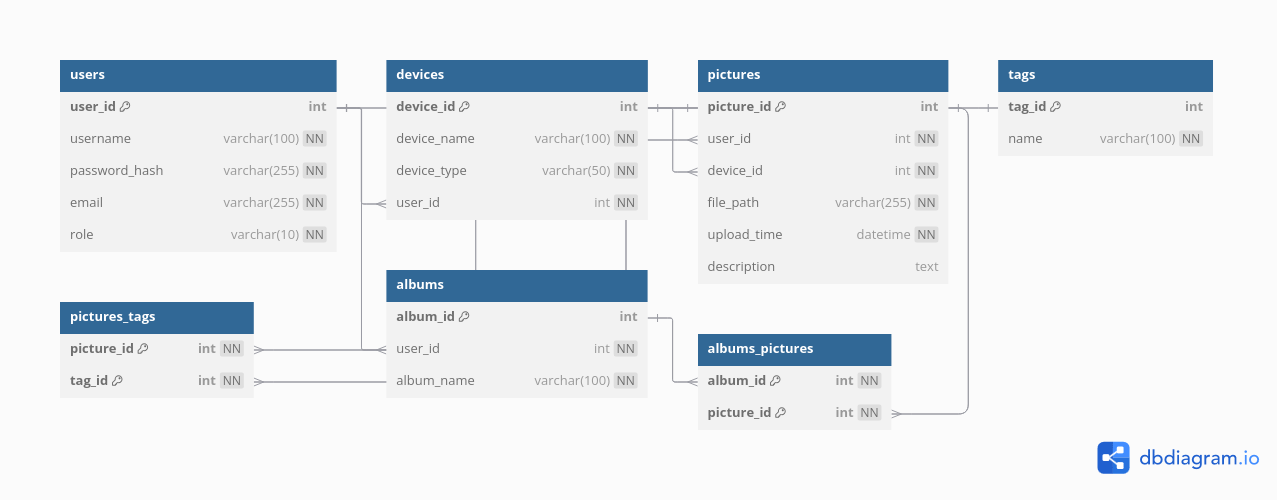
\includegraphics[width=0.8\textwidth]{diagram.png}
    %\captionof{figure}{Diagram ER dla bazy danych.}
\end{center}

\subsection{Opis tabel}
Poniżej przedstawiam opis tabel w projektowanej bazie danych.

\subsubsection{Tabela: User}
\begin{itemize}
    \item \texttt{user\_id} (PK) -- Klucz główny, identyfikator użytkownika.
    \item \texttt{username} (VARCHAR(30))-- Nazwa użytkownika.
    \item \texttt{password\_hash} (VARCHAR(255)) -- Hasz hasła użytkownika.
    \item \texttt{email} (VARCHAR(255)) -- Adres email użytkownika.
    \item \texttt{role} (ENUM('admin', 'user')) -- Rola użytkownika.
\end{itemize}

\subsubsection{Tabela: Device}
\begin{itemize}
    \item \texttt{device\_id} (PK) -- Klucz główny, identyfikator urządzenia.
    \item \texttt{user\_id} (FK) -- Klucz obcy, identyfikator użytkownika.
    \item \texttt{device\_name} (VARCHAR(50)) -- Nazwa urządzenia.
    \item \texttt{device\_type} (ENUM('kamera', 'aparat', 'smartfon', \dots)) -- Typ urządzenia.
\end{itemize}

\subsubsection{Tabela: Photo}
\begin{itemize}
    \item \texttt{photo\_id} (PK) -- Klucz główny, identyfikator zdjęcia.
    \item \texttt{user\_id} (FK) -- Klucz obcy, identyfikator użytkownika.
    \item \texttt{device\_id} (FK) -- Klucz obcy, identyfikator urządzenia.
    \item \texttt{photo\_path} (VARCHAR(255)) -- Ścieżka do pliku z obrazem.
    \item \texttt{upload\_time} (TIMESTAMP) -- Czas przesłania zdjęcia.
    \item \texttt{description} (TEXT) -- Opis zdjęcia.
\end{itemize}

\subsubsection{Tabela: Tag}
\begin{itemize}
    \item \texttt{tag\_id} (PK) -- Klucz główny, identyfikator tagu.
    \item \texttt{tag\_name} (VARCHAR(50)) -- Nazwa tagu.
\end{itemize}

\subsubsection{Tabela: PhotoTag}
\begin{itemize}
    \item \texttt{photo\_id} (FK) -- Klucz obcy, identyfikator zdjęcia.
    \item \texttt{tag\_id} (FK) -- Klucz obcy, identyfikator tagu.
\end{itemize}

\subsubsection{Tabela: Album}
\begin{itemize}
    \item \texttt{album\_id} (PK) -- Klucz główny, identyfikator albumu.
    \item \texttt{user\_id} (FK) -- Klucz obcy, identyfikator użytkownika.
    \item \texttt{album\_name} (VARCHAR(50)) -- Nazwa albumu.
\end{itemize}

\subsubsection{Tabela: AlbumPhoto}
\begin{itemize}
    \item \texttt{album\_id} (FK) -- Klucz obcy, identyfikator albumu.
    \item \texttt{photo\_id} (FK) -- Klucz obcy, identyfikator zdjęcia.
\end{itemize}

\subsection{Funkcje, Procedury, Triggery}
\begin{itemize}
    \item \textbf{Procedura składowana do przesyłania zdjęcia:} Waliduje metadane pliku, sprawdza limity użytkownika oraz wstawia nowy rekord do tabeli \texttt{Photo}.
    \item \textbf{Funkcja zwracająca statystyki użytkownika:} Zwraca ilość zdjęć, komenatrzy, tagów, itp. dla danego użytkownika.
    \item \textbf{Trigger do usuwania zdjęć:} Po usunięciu zdjęcia, usuwa również wszystkie komentarze, tagi oraz relacje z albumami.
    \item \textbf{Trigger do usuwania użytkownika:} Po usunięciu użytkownika, usuwa również wszystkie jego zdjęcia, komentarze, tagi oraz relacje z albumami.
\end{itemize}

\section{Dowód spełnienia postaci 3NF}

Aby zapewnić integralność danych oraz uniknąć redundancji, baza danych spełnia założenia 3NF.
\newline
W poniższej sekcji przedstawiam szczegółowy dowód, że projekt bazy danych opisany powyżej spełnia założenia \textbf{Trzeciej Postaci Normalnej (3NF)}. Warto pamiętać, że 3NF koncentruje się na wyeliminowaniu tzw. zależności przechodnich (transitive dependencies) oraz zapewnieniu, że atrybuty niekluczowe zależą bezpośrednio od klucza głównego (lub innego klucza kandydującego), a nie od innych atrybutów niekluczowych.

\subsection{Definicja 3NF}
Relacja (tabela) \( R \) jest w \emph{Trzeciej Postaci Normalnej (3NF)} wtedy i tylko wtedy, gdy dla każdej nietrywialnej zależności funkcyjnej
\[
X \;\rightarrow\; A
\]
spełniony jest co najmniej jeden z warunków:
\begin{enumerate}
    \item \( X \) jest \emph{superkluczem} w \( R \), czyli wyznacza wszystkie atrybuty w relacji,
    \item \( A \) jest \emph{atrybutem pierwotnym} (prime attribute), czyli należy do żadnego klucza kandydującego w \( R \).
\end{enumerate}

\subsection{Struktura tabel i zależności funkcyjne}
Poniżej przywołujemy najważniejsze tabele z określonymi kluczami głównymi oraz kluczami kandydackimi (gdzie dotyczy).

\subsubsection{Tabela: User}
\begin{itemize}
    \item \(\texttt{user\_id}\) (PK)
    \item Inne atrybuty: \(\texttt{username}, \texttt{password\_hash}, \texttt{email}, \texttt{role}\)
\end{itemize}

\noindent \textbf{Zależności funkcyjne:}
\begin{enumerate}
    \item \(\texttt{user\_id} \;\rightarrow\; (\texttt{username}, \texttt{password\_hash}, \texttt{email}, \texttt{role})\). \\
          Klucz główny (\(\texttt{user\_id}\)) wyznacza wszystkie pozostałe atrybuty, więc \(\texttt{user\_id}\) jest superkluczem.
    \item \(\texttt{username} \;\rightarrow\; \texttt{user\_id}\) (jeżeli \(\texttt{username}\) jest unikatowe). \\
          W takim wypadku \(\texttt{username}\) staje się kluczem kandydującym, a więc superkluczem.
    \item \(\texttt{email} \;\rightarrow\; \texttt{user\_id}\) (jeżeli \(\texttt{email}\) jest unikatowe). \\
          Również może pełnić rolę klucza kandydującego, a więc superklucza.
\end{enumerate}

\noindent \textbf{Wniosek (3NF):}
Wszystkie nietrywialne zależności mają po lewej stronie klucz główny lub atrybut kluczowy (superklucz). Tabela \texttt{User} jest w 3NF.

\subsubsection{Tabela: Device}
\begin{itemize}
    \item \(\texttt{device\_id}\) (PK)
    \item Inne atrybuty: \(\texttt{user\_id}, \texttt{device\_name}, \texttt{device\_type}\)
\end{itemize}

\noindent \textbf{Zależność funkcyjna:}
\[
\texttt{device\_id} \;\rightarrow\; (\texttt{user\_id}, \texttt{device\_name}, \texttt{device\_type})
\]
\(\texttt{device\_id}\) jest kluczem głównym, czyli superkluczem, więc spełnia wymogi 3NF.

\subsubsection{Tabela: Photo}
\begin{itemize}
    \item \(\texttt{photo\_id}\) (PK)
    \item Inne atrybuty: \(\texttt{user\_id}, \texttt{device\_id}, \texttt{photo\_path}, \texttt{upload\_time}, \texttt{description}\)
\end{itemize}

\noindent \textbf{Zależność funkcyjna:}
\[
\texttt{photo\_id} \;\rightarrow\; (\texttt{user\_id}, \texttt{device\_id}, \texttt{photo\_path}, \texttt{upload\_time}, \texttt{description})
\]
Klucz główny \(\texttt{photo\_id}\) jest superkluczem. Zatem warunek 3NF jest spełniony.

\subsubsection{Tabela: Tag}
\begin{itemize}
    \item \(\texttt{tag\_id}\) (PK)
    \item \(\texttt{tag\_name}\)
\end{itemize}

\noindent \textbf{Zależności funkcyjne:}
\[
\texttt{tag\_id} \;\rightarrow\; \texttt{tag\_name}
\]
\[
\texttt{tag\_name} \;\rightarrow\; \texttt{tag\_id} \quad (\text{jeżeli} \ \texttt{tag\_name} \ \text{jest unikatowe})
\]
Jeżeli \(\texttt{tag\_name}\) jest unikatowe, może ono również stanowić klucz kandydujący. W każdym przypadku lewa strona (determinant) jest superkluczem. Tabela \texttt{Tag} jest w 3NF.

\subsubsection{Tabela: PhotoTag}
\begin{itemize}
    \item Klucz główny (złożony): \((\texttt{photo\_id}, \texttt{tag\_id})\)
\end{itemize}

\noindent \textbf{Zależności funkcyjne:}
\[
(\texttt{photo\_id}, \texttt{tag\_id}) \;\rightarrow\; \dots
\]
Nie ma dodatkowych atrybutów poza kluczami obcymi, a klucz złożony (\texttt{photo\_id}, \texttt{tag\_id}) jest superkluczem. Zatem tabela \texttt{PhotoTag}\ jest w 3NF.

\subsubsection{Tabela: Album}
\begin{itemize}
    \item \(\texttt{album\_id}\) (PK)
    \item Inne atrybuty: \(\texttt{user\_id}, \texttt{album\_name}\)
\end{itemize}

\noindent \textbf{Zależności funkcyjne:}
\[
\texttt{album\_id} \;\rightarrow\; (\texttt{user\_id}, \texttt{album\_name})
\]
Klucz główny \(\texttt{album\_id}\) to superklucz. Dodatkowo, jeśli w danym modelu (\texttt{user\_id}, \texttt{album\_name}) jest unikatowe (użytkownik nie może mieć dwóch albumów o tej samej nazwie), to także jest to klucz kandydujący. W obu przypadkach determinant jest superkluczem. Tabela \texttt{Album} jest zatem w 3NF.

\subsection{Wniosek końcowy}
We wszystkich przedstawionych tabelach:
\begin{itemize}
    \item Każda nietrywialna zależność funkcyjna \((X \rightarrow A)\) ma determinanta \(X\) będącego superkluczem, \emph{lub} atrybut \(A\) jest atrybutem pierwotnym (należy do jakiegoś klucza kandydującego).
    \item Oznacza to, że nie występują zależności przechodnie, w których atrybut niekluczowy zależałby pośrednio od innego atrybutu niekluczowego.
\end{itemize}

\noindent \textbf{Konkluzja:} Wszystkie tabele w projekcie spełniają założenia \textbf{Trzeciej Postaci Normalnej (3NF)}, gwarantując tym samym zminimalizowaną redundancję danych i zwiększoną integralność informacyjną.

\section{Zabezpieczenia i Uprawnienia}
Zdefiniowano dwa poziomy dostępu do bazy danych: \textbf{Administrator} oraz \textbf{Użytkownik}. Każdy z tych poziomów ma określone uprawnienia do poszczególnych tabel.
\subsection{Administrator}
\begin{itemize}
    \item Pełne prawa: \texttt{SELECT}, \texttt{INSERT}, \texttt{UPDATE}, \texttt{DELETE} na wszystkich tabelach.
    \item Prawo do tworzenia, dropowania tabel, procedur, funkcji, triggerów.
    \item Prawo do zarządzania użytkownikami, ustawieniami aplikacji.
\end{itemize}

\subsection{Użytkownik}
\begin{itemize}
    \item Prawo do \texttt{SELECT}, \texttt{INSERT}, \texttt{UPDATE}, \texttt{DELETE} na tabelach: \texttt{User}, \texttt{Device}, \texttt{Photo}, \texttt{Album}.
    \item Brak dostępu do tabel: \texttt{Tag}, \texttt{PhotoTag}.
\end{itemize}

\section{Podsumowanie}
W powyższym dokumencie przedstawiłem projekt bazy danych dla aplikacji webowej do przeglądania i zarządzania zdjęciami użytkowników. Zdefiniowałem encje, związki między nimi, a także funkcje, procedury oraz triggery. Przedstawiłem dowód spełnienia postaci 3NF oraz zabezpieczenia i uprawnienia dla poszczególnych rodzajów użytkowników.

\end{document}
